Ice in the ocean is part of the ocean. In the case of sea ice it comes from sea water that freezes as it is cooled by a cold atmosphere, with some addition of snow accumulating on the top. In the case of icebergs, it generally comes from glaciers that feeds the ocean with pieces of ice that is compacted snow that has fallen on continents, and contains no salt. 

The interaction of waves and ice is a subject that is very complex. It is made more difficult by  the paucity of available measurements. Fortunately, research efforts have been amplified since 2010, in an area where much is still to be discovered. These efforts are motivated by the rapid evolution and poor climate projections of the sea ice cover, in particular in the Arctic. Sea ice has an important role in isolating the ocean from the atmosphere and solar radiation, effectively shutting off heat and gas fluxes and increasing the ocean albedo. As a result, the effects of waves, pushing the ice or enhancing  ice formation and melting, are important for understanding the ice edge dynamics and air-sea interaction from weather forecasting to climate projections. Another reason for studying waves in ice, is that the emerging Arctic ocean is a place of increased human activities, with new shipping routes and increasing exploitation of natural  resources. As a result, any activity there requires the development of wave forecasting capabilities, in particular around the ice edge. 

This chapter discusses several key processes of wave-ice interactions, starting with sea ice and finishing with icebergs which is made special by its very large thickness. 
In all of these processes , one obvious aspect is that ice is a solid that floats, but a solid that can take many shapes and forms. Ice also deforms, and can break into pieces under the strain caused by ocean waves.
Although we start with an account of frazil and pancake ice, it should be remembered that these are probably not the most common ice form. Still, it is estimated that 50\% of the Antarctic ice \citep{Gow&al.1982}, and less so in the Arctic,  is initially grown as frazil and pancakes. Hence, this early stage of development is a very important one. 

Without going in too many details about the physical properties of ice and its consequences for sea ice \citep[see][]{Weeks2010}, it is important to note that sea water freezing results in the formation of cristals of pure ice that then confine salt to brine pockets and a few other cristals involving, among other carbonates. Also, the freezing of water with salinity above 25 PSU produces sea ice with low salinity (typically 10--20 PSU, made up of ice cristals and brine) and increases the salinity of the surrounding water. That more saline water is denser and will thus lead to some convection in the upper ocean mixed layer. If the original water is brackish (defined here with a salinity under 25 PSU) then the more salty water is less dense, and will be stably floating on less salty water, so that ice formation can develop in a very thin surface layer \citep[][p. 48]{Weeks2010}. Here we will not discuss these brackish conditions that are specific to large Arctic estuaries. 

When the water is very calm it freezes from the surface as columnar ice crystals, forming large slabs of congelation ice. The wave-induced perturbation facilitates the nucleation of ice cristals that grow into a suspension of small platelets of ice, known as frazil ice.  Due to their buoyancy, these frazil cristals concentrate at the sea surface, like a snowstorm flipped upside down. 

%%%%%%%%%%%%%%%%%%%%%%%%%%%%%%%%%%%%%%%%%%%%%%%%%%%%%%%%%%%%%%%%%%%%%%%%
\begin{figure}[htb]
\centerline{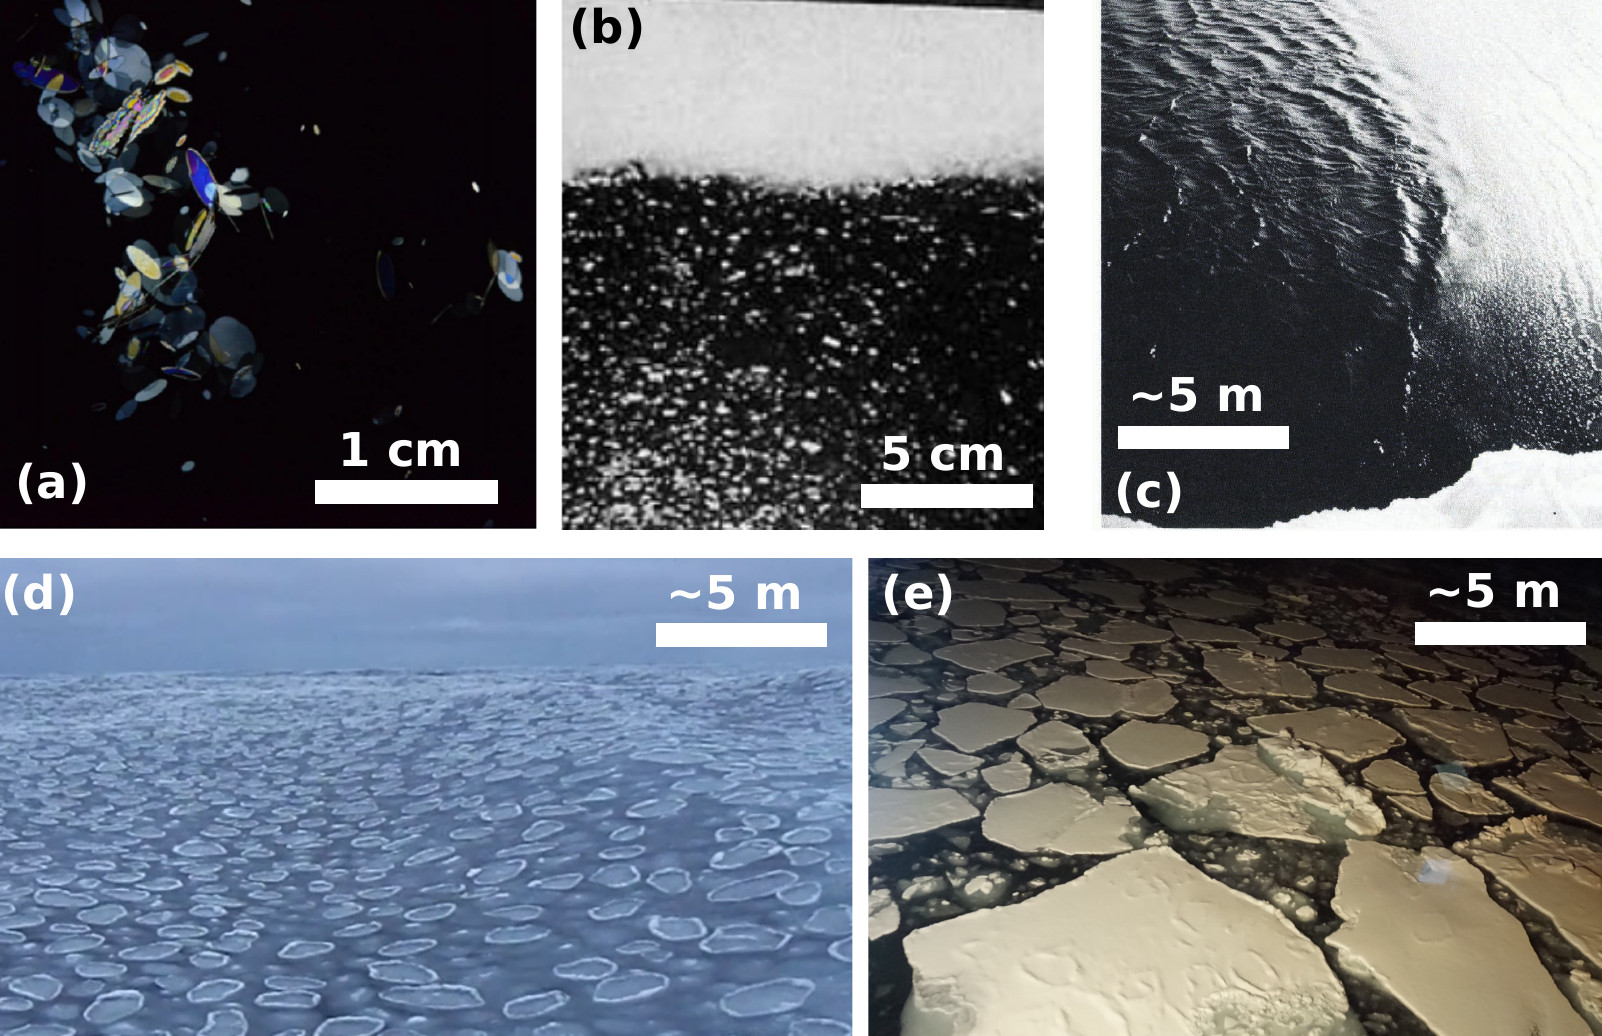
\includegraphics[width=\textwidth]{FIGURES/ice_frazil_pancakes.jpg}}
  \caption{From frazil to pancakes.}{(a) vertical plane view of frazil cristals viewed with polarized light, and their aggregation (copyright Elsevier, taken from \cite{McFarlane&al.2015}. (b) accumulation of frazil in a surface layer under waves. (c) Formation of an ice edge in frazil ice \citep[From][, copyright Cambridge University Press]{Martin&Kauffman1981}. (d) Field of pancakes in a storm as recorded by E. Rogers on October 12, 2015 in the Beaufort sea \citep{Rogers&al.2016}. (e) Ice floes resulting from the agregation of pancakes, Beaufort sea, November 1, 2015, picture by H. Shen.} \label{fig:frazil_pancakes}
\end{figure}
%%%%%%%%%%%%%%%%%%%%%%%%%%%%%%%%%%%%%%%%%%%%%%%%%%%%%%%%%%%%%%%%%%%%%%%%


\section{From water to pancakes}
\subsection{Suspensions of frazil cristals and effective viscosity}
Knowledge on frazil properties mostly come from laboratory experiments, such as those performed by  \cite{Martin&Kauffman1981}, in which sea water in a wave tank is cooled. As sea water approaches the freezing temperature, around -2$^\circ$ C for a salinity of 35 PSS, disk-shaped ice cristals form with diameters 1--3 mm and thickness of 1 to 10 micrometers, as shown in figure \ref{fig:frazil_pancakes}.a. The volume concentration $\phi$ of this suspension may vary in the range  $0.15<\phi<0.45$ depending on the confinement of the water. In particular, the dissipation of waves by the ice induces a compression force due to the convergence of the wave momentum flux. This wave-induced force tends to increase the concentration at the ice edge exposed to the waves. 

Such a concentration of solid particles enhances the effective kinematic viscosity $\nu_1$ of the suspension compared to that of the fluid component only which, at the freezing point is $\nu_w \simeq 1.83 \times 10^{-6}$~m$^2$~s$^{-1}$. The ratio $\nu_1/\nu_w$ for a concentrated solution of solid glass spheres 
is expected to vary like \citep{Mooney1951}
\begin{equation}
\frac{\nu_1}{\nu_w} = \exp \left[2.5 \phi /(1-1.43 \phi)\right].\label{eq:visc_Mooney}
\end{equation}
 This equation gives a factor 2 at $\phi=0.2$ and a factor 23 at $\phi=0.45$. 
 
Representing the ocean as a two layer system with different viscosities, $\nu_1$ for the top layer of thickness $h_1$, and $\nu_w$ for the underlying and deep layer, wave attenuation is exponential. A first approximate solution was given by \cite{Weber1987} with a very large viscosity in the surface layer gave a dissipation dominated by the viscosity of the underlying water, independently of the top layer viscosity and thickness, identical to the solution by 
\cite{Dore1978} for the viscous friction at the air-sea interface. The general solution, including finite depth of the underlying layer is given by \cite{Keller1998}. The resulting dissipation can be very strong for waves relatively short compared to the frazil layer, which explains the strong attenuation of waves in figure \ref{fig:frazil_pancakes}.c. However, longer waves are not much attenuated once their wavelength is much larger than $h_1$. 

%GIVE SIMPLIFIED IMAGINARY K HERE . 
 
 Now, the empirical coefficient 1.43 in Mooney's eq. (\ref{eq:visc_Mooney}) is strongly dependent on the solid material that is in suspension. 
Besides, the frazil cristals are not spherical and, for smaller wave amplitudes, these disks tend to stick together \citep{Martin&Kauffman1981}. 

The problem of flat ellipsoids in suspension, instead of spheres, was addressed by \cite{deCarolis&al.2005}, who give an effective viscosity in the form of a power law  
\begin{equation}
\frac{\nu_1}{\nu_w} = (1- \phi)^K.
\end{equation}
Interpreting the wave attenuations measured by \cite{Martin&Kauffman1981}, \cite{deCarolis&al.2005} find 
that the exponent $K$ is of the order of 15 to 20 to explain the effective viscosities in the range 0.002--0.01~m$^2$~s$^{-1}$. They conclude that such high values can only be explained by a dominance of solid-solid interactions, including 
collisions, friction and some sticking, and these all very sensitive to strain rate. It is thus expected that the effective viscosity is generally a non-linear function of the strain rate and volume concentration. 

As pointed out by \cite{Martin&Kauffman1981}, the thickness and concentration of grease ice is modulated by wave-generated roll structures known as Langmuir circulations (see chapter \ref{ch_ioa}). The ice collects in the surface convergence zone of these rolls. \cite{Garrett1976} had envisaged that a  localized wave dissipation in the convergence zone, in his case due to wave breaking over the stronger current, could reinforce the rolls. The stronger dissipation due to thicker grease ice could play the same role. These effects may be relevant for the enhancement of air-sea fluxes in leads \citep{Esau2007}.

%\cite{Newyear&Martin1997} : unrealistic uniform viscosity.


\subsection{Pancake ice}
Natural grease does not remain a suspension of ice fragments of similar sizes and shapes. Instead, grease ice evolves to the formation of pancakes. These are agglomerations of frazil that weld together. Once a pancake has started forming, it can grow by the washing of frazil ice over the top of the pancake and its subsequent freezing \citep{Doble&al.2003}. The raised rim of the pancakes, clearly visible as a white skirt in figure \ref{fig:frazil_pancakes}.c, come from their mutual collisions. Pancakes typically grow to diameters of the order of 1 m, and the ocean can be covered by a few layers of a pancakes. \cite{Shen&al.2001} discussed that the maximum diameter of the pancakes observed in the laboratory is generally of the order of 1\% of the  the dominant wavelength, possibly due to break-up by bending or stretching if the pancakes get larger. This scaling of the pancake diameter with the wavelength was also confirmed by \cite{Roach&al.2018} with video acquired in the Beaufort Sea, but they could not conclude if bending or stretching was the main mechanism that limits the size of pancakes. 

Pancakes have thicknesses that rarely exceed a few centimeters, so that they easily raft and form a an ice layer with several pancakes irregularly stacked. The dissipation of energy in this ice layer is certainly dominated by ice-ice friction and collisions. Even though the local surface motions is consistent with orbital wave motion without ice (the ratio of horizontal to vertical motions recorded by buoys is very close to 1), there is a very strong dissipation of short wave components. Several models have been proposed to represent this dissipation, ranging from the viscous layer model of \cite{Keller1998}, to more complex visco-elastic models \citep{Wang&Shen2010,Rogers&al.2016}. These latter models include different modes of motion and \cite{Mosig&al.2015} show that some of these are often similar to what is predicted by a viscous thin beam model. Unfortunately, all these models are highly empirical, and there is no method for determining a priori the viscosity and elasticity parameters from large scale environmental conditions. 

\section{Dispersion relations}
Whereas the condition of zero pressure at the free surface  and the horizontal momentum balance gives the usual ice-free dispersion relation $\sigma^2 = g k \tanh(kD)$, the presence of ice clearly modifies these two conditions and thus the dispersion relation. A first effect, when ice is not broken in floes shorter than the wavelength, is the resistance to stretching of the sea surface. This same effect is similar to the effect of surface tension, and thus also leads to an increase of the phase speed for the shorter waves. 
One parameterization of that effect uses a flexural rigidity $L$, and gives the dispersion relation 
\begin{equation}
L k^5= \rho_w (g - \sigma^2 h_i  \rho_i/\rho_w )k - \rho_w \sigma^2
\end{equation}

 Otherwise, if the ice sheet is broken up in pieces, there is only the effect of the added ice mass, as given by \cite{Fox&Haskell2001}, in which case the phase speed is decreased by the presence of ice, 
\begin{equation}
k= \frac{\sigma^2}{g - \sigma^2 h_i  \rho_i/\rho_w }.
\end{equation}

There are many more complex theories for the dispersion relation \citep[e.g.][]{Meylan&al.2018} that can give faster of slower phase speeds depending on conditions.  The observations generally find faster propagation for short waves over thick ice, compared to waves without ice, for example for waves periods shorter than 12~s in 1.5~m thick ice \citep{Marsan&al.2012}. In the case of 0.3~m thick floes, \cite{Fox&Haskell2001} instead found a slower phase speed (compared to waves without ice) for periods in the range 6 to 8~s (they did not measure shorter waves).  

 
\section{Dissipation for solid floes: basal friction}
When freezing persists, pancakes weld together, leading to a single and continuous layer of ice. The agitation due to waves that has led to the formation of pancakes results in a thicker layer of ice compared to freezing conditions without agitation that produces columnar ice in which the heat is lost to the atmosphere by diffusion through the ice layer. 

With such a single ice layer heaving up and down with the wave motion but constrained in its horizontal displacement, the dissipation energy can occur in the boundary layer below the ice. This oscillatory boundary layer is similar to the air-side boundary layer discussed in section \ref{Dore1978}, and the bottom boundary layer discussed in chapter \ref{ch_wbbl}. For the case of ice, the problem was treated by \cite{Liu&MolloChristensen1988}, with the additional effect of ice inertia that we neglect here. Here we consider the finite viscosity of seawater at the freezing point, $\nu_w \simeq 1.83 \times 10^{-6}$~m$^2$~s$^{-1}$. For monochromatic waves of radian frequency $\sigma$,  a boundary layer of thickness $\sqrt{\nu_w \sigma}$ develops in the laminar case, and the attenuation rate of the wave energy in time is 
\begin{equation}
\beta_{\mathrm{ice,bfr,v}}=-k\sqrt{\nu_w \sigma / 2}.  \label{eq:beta_ice_visc}                                                                                                                                                                                                                                                                                                                                                                                                                                                                                                                                                                                                                                                                                                                                                                         
\end{equation}
This is the same dissipation rate that was found by \cite{Phillips1977} for waves under an inextensible layer of oil \citep[see also][]{Weber1987}.
For a smooth under-ice surface, if we accept the similarity with the bottom boundary layer, this laminar regime is expected to occur for Reynolds numbers $\mathrm{Re} = \sigma a^2/\nu < \mathrm{Re} _c$, with $\mathrm{Re} _c=1.5 \times 10^5$ \citep{Jensen&al.1989}. Above this value the boundary layer transitions into a turbulent regime. In that case the dissipation rate becomes quadratic,
\begin{equation}
\beta_{\mathrm{ice,bfr,t}}=-f_e u_{\mathrm{orb}} / g,\label{eq:beta_ice_turb}
\end{equation}
where $u_{\mathrm{orb}}$ is is the significant orbital velocity amplitude at the water-ice interface. 
The dissipation factor $f_e$ is obtained from the under-ice roughness in the same way that it was obtained in the turbulent bottom boundary layer in chapter \ref{ch_wbbl}.

For random waves, neglecting the effects of the 
ice layer on the water motion, we use the solution given in chapter \ref{ch1b}, 
\begin{equation}
u_{\mathrm{orb}}= 2\sqrt{\int_0^\infty \frac{\sigma^2}{\tanh^2(kD)} E(f) \mathrm{d}f },
\end{equation}
with a significant horizontal displacement
\begin{equation}
a_{\mathrm{orb}}= 2\sqrt{\int_0^\infty  \frac{1}{\tanh^2(kD)}E(f) \mathrm{d}f },
\end{equation}
and we use this definition of the Reynolds number, $\mathrm{Re} = u_{\mathrm{orb}} a_{\mathrm{orb}} /\nu$.

Because the superposition of linear waves gives a Rayleigh distribution of the amplitudes, the transition between laminar and turbulent 
can happen only for the highest waves, giving a smooth transition of the average dissipation rate $\beta_c$. In practive, considering a Rayleigh distribution gives a value of $\beta_c$ that is very close to the following approximation 
\begin{equation}
\beta_c= (1-w)  \beta_{\mathrm{ice,bfr,v}} + w \beta_{\mathrm{ice,bfr,t}},\label{eq:beta_c_ice_bfr}
\end{equation}
as shown in figure \ref{fig:under_ice_friction}, where we have used a weight $w=0.5 \left[1 + \tanh((\mathrm{Re}-\mathrm{Re}_c)/\Delta_{\mathrm{Re}}\right]$, and $\Delta_{\mathrm{Re}}=2 \times 10^5$.
%%%%%%%%%%%%%%%%%%%%%%%%%%%%%%%%%%%%%%%%%%%%%%%%%%%%%%%%%%%%%%%%%%%%%%%%
\begin{figure}[htb]
\centerline{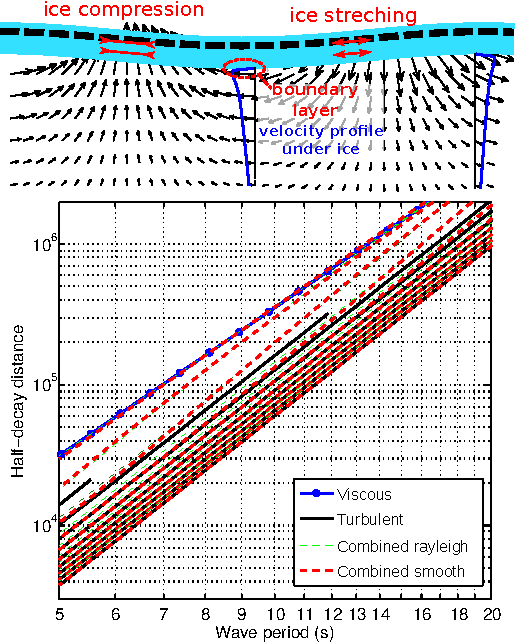
\includegraphics[width=0.65\textwidth]{FIGURES/under_ice_friction_laminar_turbulent.pdf}}
  \caption{Top: schematic of velocities and boundary layer below an ice layer (light blue). Bottom: expected decay distance $X_{1/2}=C_g \ln(2)/\beta_c $ as a function of wave period $T$, for an under-ice roughness of 0.1~mm, and wave heights ranging from 0.5 to 5~m. The `combined Rayleigh' solution uses a combination of $\beta_{\mathrm{ice,bfr,v}}$ and $\beta_{\mathrm{ice,bfr,t}}$ with a weighting depending on a Rayleigh distribution of wave amplitudes, and the `combined smooth' solution is given by eq. (\ref{eq:beta_c_ice_bfr}). Adapted from \cite{Stopa&al.2016}.} \label{fig:under_ice_friction}
\end{figure}
%%%%%%%%%%%%%%%%%%%%%%%%%%%%%%%%%%%%%%%%%%%%%%%%%%%%%%%%%%%%%%%%%%%%%%%%

It should be noted that even the laminar dissipation is relatively strong, with half-decay distances under 400~km for periods shorter than 10~s, and 30~km under 5~s. This viscous dissipation is larger than what was estimated from buoys in pancake ice in recent experiments \citep{Ardhuin&al.2018b}. \cite{Rogers&al.2016} reported imaginary wavenumbers $k_i = 2 \ln(2) / X_{1/2}$ of the order of $2 \times 10^{-5}$ for a period $T=5$~s, which corresponds to $X_{1/2} = 140$~km, 4 times larger than due to molecular viscosity under an inextensible surface ice sheet. This is possible because the pancakes actually move horizontally and raft to form multiple layers, so that the present theory for $\beta_c$ gives an overestimate of the wave dissipation in pancake ice. In the case of densely packed thick floes, rafting does not occur and the horizontal ice motion is much weaker than the vertical motion \citep{Fox&Haskell2001}, in which case the above expression for $\beta_c$ should be applicable.

\section{Dissipation for solid floes: flexure and the importance of ice break-up}
In other cases, under-ice friction appears insufficient to explain the observed attenuation. This is particularly the case for the large-scale attenuation of  swells with periods 18 to 33~s reported by \cite{Ardhuin&al.2016}, and illustrated in figure \ref{fig:TARA_data_model}. In that study of waves measured in the pack, 1500~km from the ice edge, the constant dissipation rate needed to obtain a reasonable agreement with the data corresponds to a spatial decay of the energy, $\alpha=\beta/C_g$, ranging from $\alpha \simeq 4 \times10^{-6}$~m$^{-1}$ at $T=20$~s, to $\alpha\simeq 2 \times 10^{-6}$~m$^{-1}$ at $T=25$~s.
These are 12 times the effect of viscous friction below a smooth ice plate as given by eq. (\ref{eq:beta_ice_visc}). 
That seems impossible to explain by the ice morphology alone, with complicated keel structures, often exceeding 10 m below the mean ice level \citep{Doble&al.2011}.

%%%%%%%%%%%%%%%%%%%%%%%%%%%%%%%%%%%%%%%%%%%%%%%%%%%%%%%%%%%%%%%%%%%%%%%%
\begin{figure}[htb]
\centerline{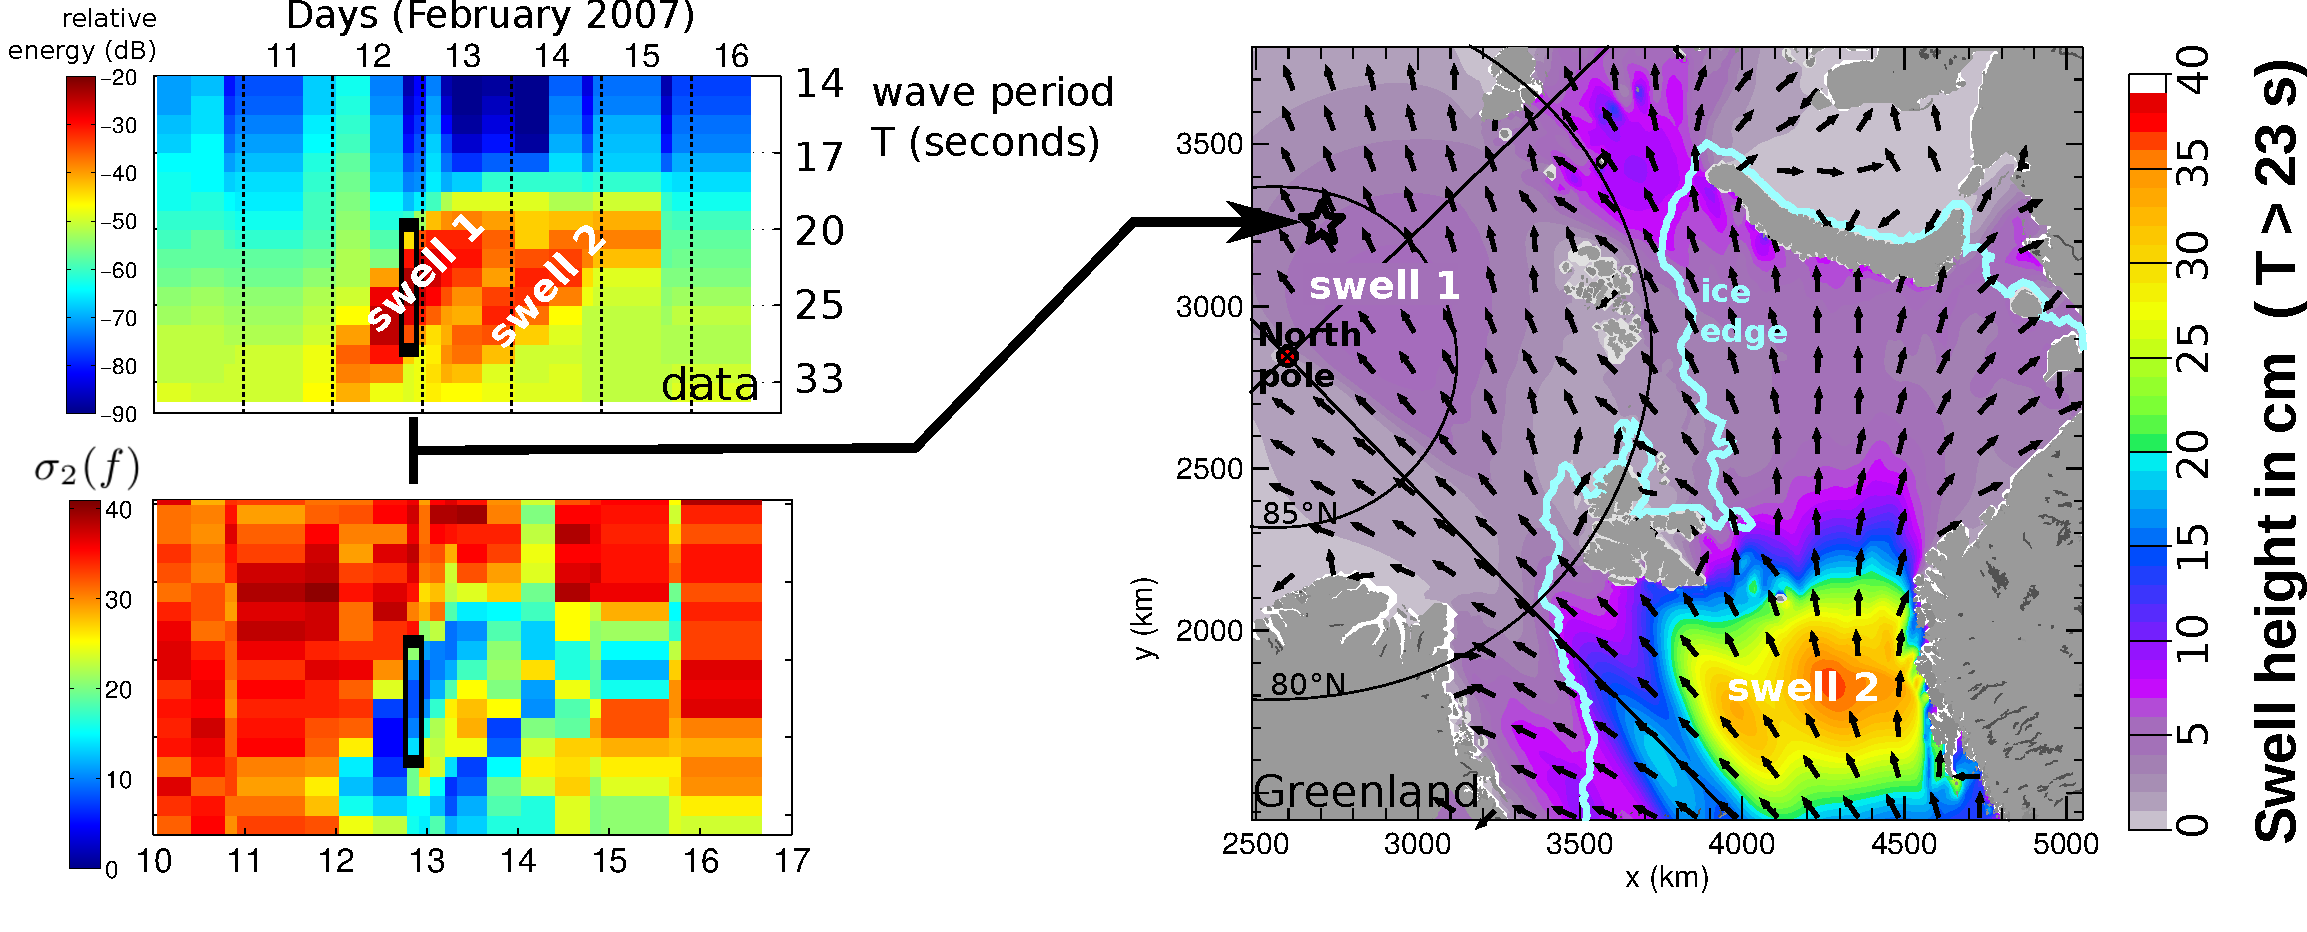
\includegraphics[width=\textwidth]{FIGURES/TARA_data_model.pdf}}
  \caption{Left: Spectrogram of surface elevation and width  $\sigma_2$ of the directional 
wave spectrum estimated from second moments $a_2$ and $b_2$.  The black rectangle highlights the time and frequency range of the spectral peak on February 12 at 18:00 UTC, showing that the directional spreading is around 10$^\circ$ or less when the energy is maximum. Right: model snapshot giving some context to the measured data. The two swell events are due to two distinct storms. Adapted from \cite{Ardhuin&al.2016}.} \label{fig:TARA_data_model}
\end{figure}
%%%%%%%%%%%%%%%%%%%%%%%%%%%%%%%%%%%%%%%%%%%%%%%%%%%%%%%%%%%%%%%%%%%%%%%%


Also, dissipation by basal friction leads to unrealistic high values of swell heights, of a few centimeters, crossing the Arctic from Fram Strait to Alaska \citep{Ardhuin&al.2016}. For this reason, the dissipation of energy associated to the deformation of the ice was studied by \cite{Ardhuin&al.2018b,Boutin&al.2018,Ardhuin&al.2020}. Several dissipation effects have been studied in the laboratory and in the field, they include anelastic effects \cite{Cole1995,Cole&al.1998} and inelastic effects, related to dislocations at large strain rates \citep{Cole&Durell2001}.  These effects are consistent with a strong reduction in wave attenuation as soon as the ice is broken up  \citep{Ardhuin&al.2020}, and may explain the very wide range of attenuations found in 
remote sensing data across Antarctic sea ice by \cite{Stopa&al.2018b}. 



\section{Scattering of waves by sea ice}
Alternatively, following early experiments in the the Arctic \citep{Wadhams&al.1986}, it was proposed that the multiple reflections at the edges of ice floes, or at sharp gradients in ice thickness, could be a significant of source of attenuation, similar to the Bragg scattering of waves by bottom topography that is described in chapter \ref{ch5}. The ice-induced "scattering" has been the subject of many theoretical works \citep{Squire2020}. When scattering is the dominant source of wave attenuation in the sea ice it should be associated with a strong broadening of the wave directional spectrum, with a wave spectrum becoming nearly isotropic near the ice edge.  There is, however, very little support for a general broadening of wave spectra in sea ice.  \cite{Sutherland&Gascard2016} found a minor increase in directional spread off the East coast of Greenland, but that is not sufficient to explain most of the wave amplitude attenuation. 

Over the scale of the Arctic basin, the example shown in Fig. \ref{fig:TARA_data_model} clearly disproves the idea that there is a significant scattering of swells by under-ice topography, which was proposed by \cite{Squire&al.2009}. In the marginal ice zone, all remote sensing data, except in cases of crossing seas \citep{Ardhuin&al.2015b}, show long-crested swells that are not compatible with a strong scattering. 
%\section{Feedbacks of sea ice formation and melt}
%\cite{Sutherland&Dumont2018}, \cite{Stopa&al.2018}

\section{Waves and icebergs}
%%%%%%%%%%%%%%%%%%%%%%%%%%%%%%%%%%%%%%%%%%%%%%%%%%%%%%%%%%%%%%%%%%%%%
\begin{figure}%[htb]
\begin{center}
 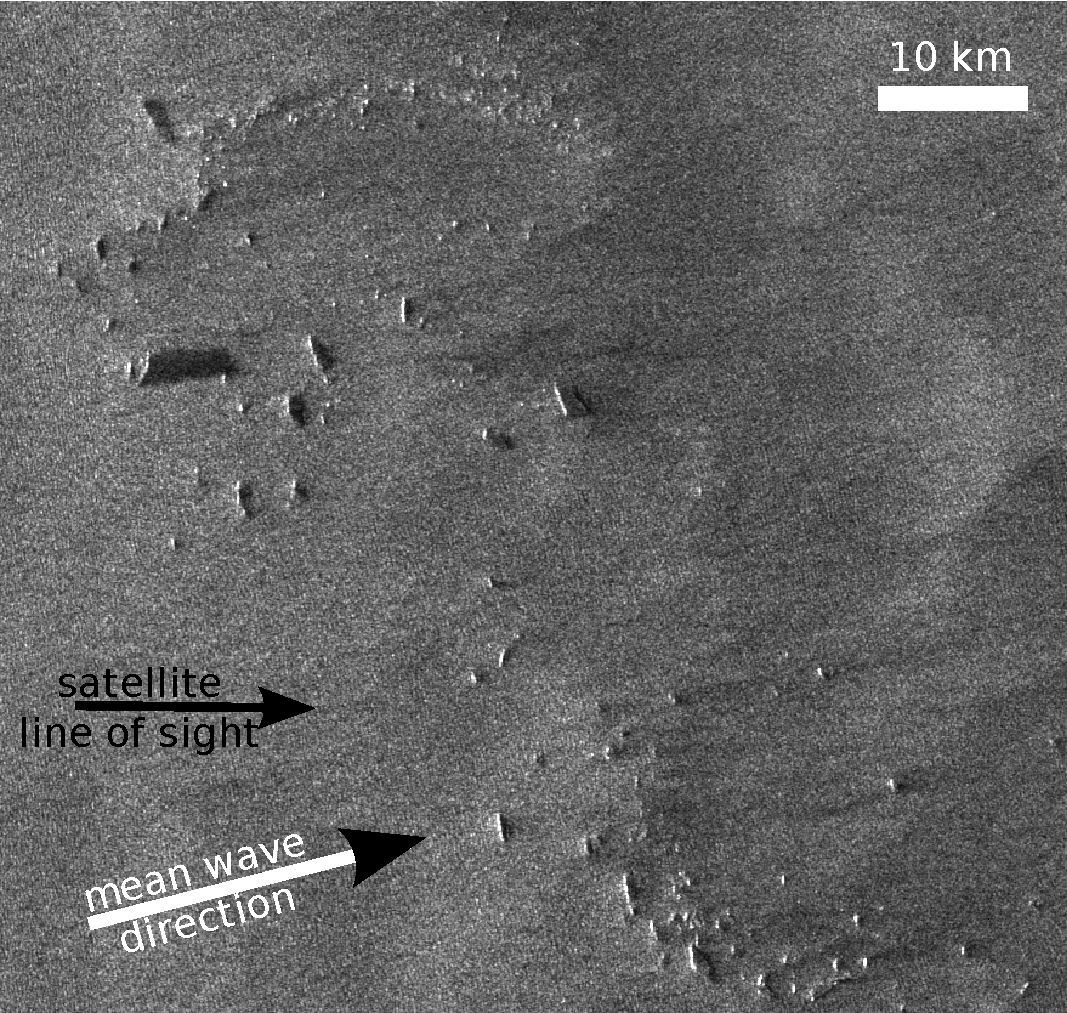
\includegraphics[width=0.7\columnwidth]{FIGURES/SAR_icebergs.pdf}
 \caption{Example of a synthetic aperture image acquired by Envisat's ASAR instrument at 
53$^\circ$S 155$^\circ$W on December 26, 2008, 9:35 UTC. White areas are the sides of icebergs facing the satellite.
Waves propagate from the West (left of the image, see arrow) and a majority of icebergs align their 
longer sides in the North-South direction. The dark areas to the right of bright spots are either the body of iceberg in or the sea surface in the radar shadow 
behind the iceberg (narrow strips next to the iceberg), or areas with low wind and/or greasy ice for which the backscatter is very low. 
A few icebergs are almost square tabular bergs with their top seen in an intermediate grey level between the very bright illuminated sides and the darker modulated
sea. The ``short'' modulations (with a 270~m wavelength) in the grey level throughout the image are the ocean waves. Only 25\% of the 
full image is shown.\label{fig:SAR_icebergs}}
 \end{center}
\end{figure}
%%%%%%%%%%%%%%%%%%%%%%%%%%%%%%%%%%%%%%%%%%%%%%%%%%%%%%%%%%%%%%%%%%%%%
Either at large ice shelves around Antarctica or from smaller glaciers around Greenland, icebergs are formed by the calving of ice streams reaching the oceans. Large icebergs are found in the Southern Ocean, with the largest ever observed having the same area as Belgium. Recent large calving events from the Larsen ice shelf have attracted headlines, but there are thousands of icebergs a few kilometers in diameter \citep{Tournadre&al.2016} that deserve attention because they are the ones that give the largest "cross-section" for incoming waves, and are responsible for very strong wave attenuation in the Southern Ocean \citep{Ardhuin&al.2011b}. Indeed, these floatings islands of ice act like giant break-waters. At present we only have a statistical knowledge of their presence, with a monthly database of their occurence developed by Ifremer \citep{Tournadre&al.2016}. 


As a result, the average estimated impact of these icebergs can be a reduction in wave height that exceeds 0.5~m over vast regions of the Southern Ocean and is highly variable in time as clusters of "small" icebergs are caused by the break-up of the largest calved icebergs. In particular, the anomalously large number of small icebergs in the South Pacific in 2008 is related to the breakup of iceberg C19a \citep{Tournadre&al.2012}.

%%%%%%%%%%%%%%%%%%%%%%%%%%%%%%%%%%%%%%%%%%%%%%%%%%%%%%%%%%%%%%%%%%%%%
\begin{figure}%[htb]
\begin{center}
 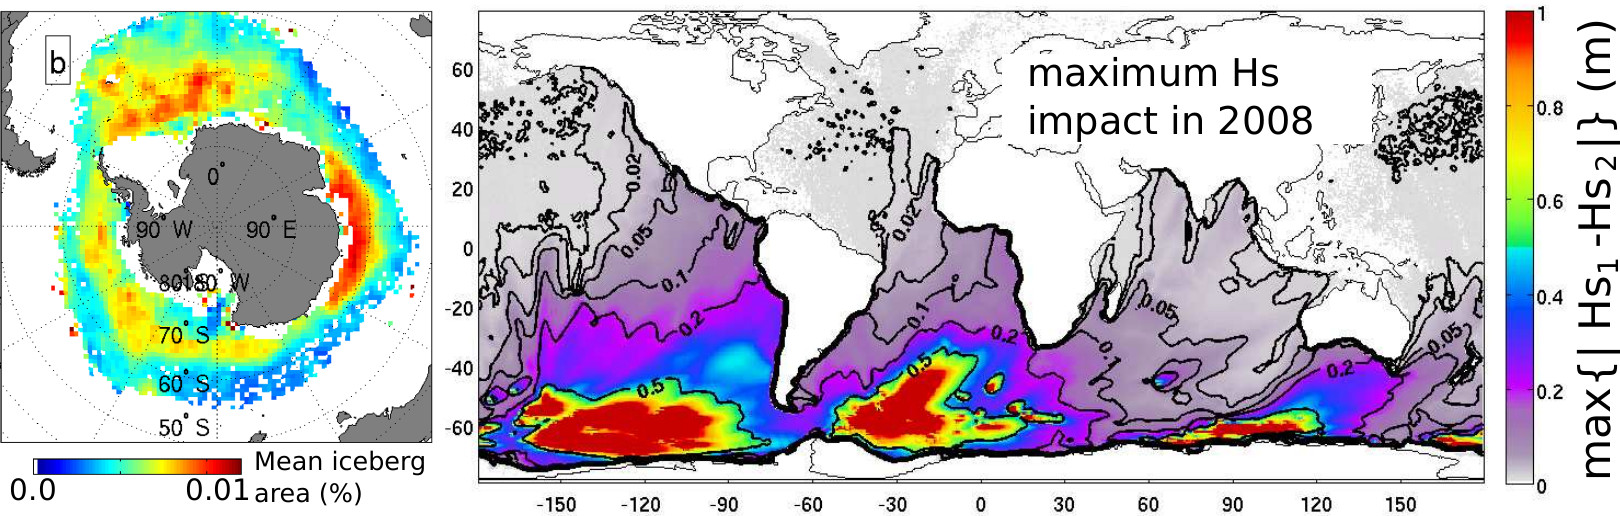
\includegraphics[width=\columnwidth]{FIGURES/model_icebergs.jpg}
 \caption{Left: climatological mean of the fraction of ocean area covered by icebergs. Right: maximum difference, in meters, over the year 2008, between modeled wave heights without ($Hs_1$) 
and with ($Hs_2$) icebergs parameterized using the Ifremer database. Reproduced from \cite{Ardhuin&al.2011b}.\label{fig:iceberg_model}}
 \end{center}
\end{figure}
%%%%%%%%%%%%%%%%%%%%%%%%%%%%%%%%%%%%%%%%%%%%%%%%%%%%%%%%%%%%%%%%%%%%%
%\subsection{Floating breakwaters}
%\cite{Ardhuin&al.2011b}
%\subsection{Iceberg break-up and erosion caused by waves}
%\cite{Wagner&al.2018}
